\documentclass{standalone}
\usepackage{tikz}
\usepackage{ctex,siunitx}
\usepackage{tkz-euclide}
\usepackage{amsmath}
\usetikzlibrary{patterns, calc}
\usetikzlibrary {decorations.pathmorphing, decorations.pathreplacing, decorations.shapes,}
\begin{document}
\small
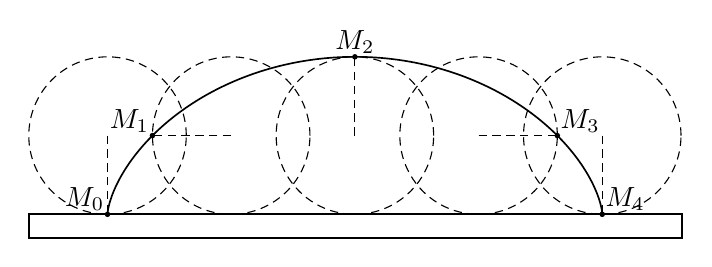
\begin{tikzpicture}[>=latex,scale=1.0,inner sep=1pt]
  \foreach \x/\y in {0/above left,1/above left,2/above,3/above right,4/above right}
    { 
      \draw[densely dashed](0.5*pi*\x,1)circle(1);
      \fill([shift=(-\x*90-90:1)]0.5*pi*\x,1)circle(1pt)node[\y]{$M_\x$};
      \draw[densely dashed](0.5*pi*\x,1)--++ (-\x*90-90:1);
    }
  \draw[semithick,domain=0:360,samples=200] plot ({\x/180*pi-sin(\x)},{1-cos(\x)});
  \draw[thick](-1,0)rectangle(7.3,-0.3);
\end{tikzpicture}
\end{document}